% https://tex.stackexchange.com/questions/58878/tikz-set-node-label-position-more-precisely
\documentclass[12pt]{standalone}

\usepackage{fontspec}
  \setmainfont{tex gyre termes}
\usepackage{tikz}
\usepackage{amsmath}
\newcommand{\xMin}{-3}%
\newcommand{\xMax}{+3}%
\newcommand{\yMin}{-3}%
\newcommand{\yMax}{+3}%

% GNUPLOT required
\begin{document}
\pagestyle{empty}

  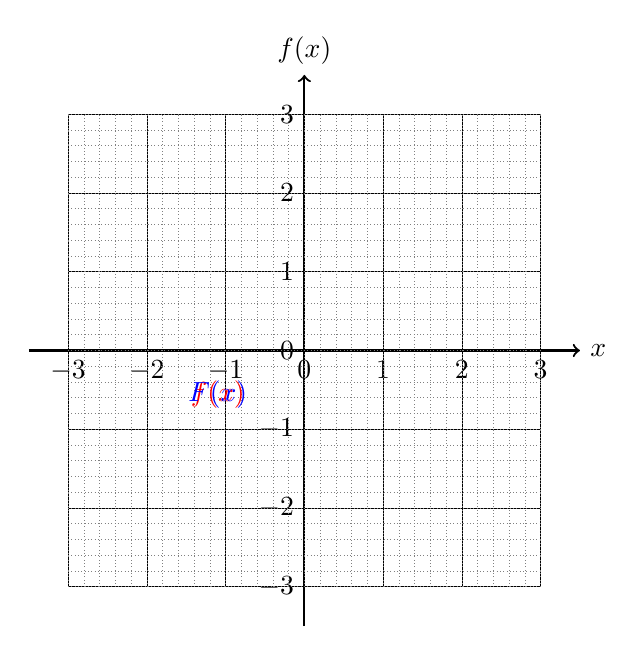
\begin{tikzpicture}[domain=\xMin:\xMax,samples=10000]
    \draw[thick, ->] (\xMin-0.5,0) -- (\xMax+0.5,0) node[right] {\(x\)};
    \draw[thick, ->] (0,\yMin-0.5) -- (0,\yMax+0.5) node[above] {\(f(x)\)};

    \foreach \i in {\xMin,...,\xMax} {
      \draw [very thin,black] 
        (\i,\yMin) -- (\i,\yMax) node [below] at (\i,-0.01) {$\i$};
    }
    \foreach \i in {\yMin,...,\yMax} {
      \draw [very thin,black] 
        (\xMin,\i) -- (\xMax,\i) node [left] at (-0.01,\i) {$\i$};
    }
    \draw[very thin, densely dotted, color=gray, step=0.2] (\xMin,\yMin) grid (\xMax,\yMax);

    \draw[color=red,  thick] plot[id=f] function{2*x*sin(1/x)-cos(1/x)}
      node[label={[xshift=-1.1cm, yshift=-1cm] \(f(x)\) }] {};
    \draw[color=blue, thick] plot[id=F] function{(x*x)*sin(1/x)}
      node[label={[xshift=-1.1cm, yshift=-1cm] \(F(x)\) }] {};  
  \end{tikzpicture}
\end{document}